\chapter{Model validation and setup}

Refer to work of Grogger that investigated deep propagating GWs, individual spectral forcings, linear analysis vs numerical results...

Grogger also showed EULAG simulations for transient lower boundary, more specifically growing amplitude / rising topography 

extend with the comparing numerical to analytical results of GWD for different MW regimes...
and show transient lower boundary moving in x-direction


\section{Reproducing results from linear theory for different MW regimes with non-linear numerical simulation}

% Show analysis plots for one simulation and then result of drag for all

One established approach to validate a numerical model is the comparison of non-linear numerical simulations to results from linear theory. For the investigation of GWs and corresponding processes drag values and momentum flux distributions are suitable.

% - \textcite{blumen} (Blumen 1965a, Fig. I)

- \textcite{bretherton_momentum_1969}

- \textcite{smith_influence_1979} looked circular bell-shaped mountain? only looks at 2D flow of stratified rotating fluid! Flow is independent of y coordinate! 

- Smith assumes symmetric mountain and only looks at one dimension in spectral space?? assumes geostrophic flow? uses gaussian quadrature or bessel functions...

- dimensionless drag is specified differently for Smith and miranda due to additional dimension

- \textcite{miranda_non-linear_1992} obtained the wave drag in a more general non-hydrostatic rotating case and derived an analytic solution for the hydrostatic rotating limit circular bell-shaped mountain. 

- integrate over two dimensions and assume a cross-section with V=0 to calculate drag. Keeps 3D problem first -> equations different to Smith, ...?

- W.K.B


\begin{table*}[ht]
\centering
\caption{Parameters for numerical simulations of different MW regimes: mountain width L, spatial increments $\Delta$x and $\Delta$z in the horizontal and vertical directions, time step $\Delta$t, thickness $\delta$x$_{ab}$ and time scale $\tau_x$ of the horizontal and altitude z$_{ab}$ and time scale $\tau_z$ of the vertical absorbers.}

\begin{tabular}{@{}cccccccc@{}}
\toprule
L/km & $\Delta$x/m & $\Delta$z/m & $\Delta$t/s & $\delta$x$_{ab}$/km & $\tau_x$/s  & z$_{ab}$/km & $\tau_z$/s \\ \midrule[1pt]

1   & 50  & 50 & 5   & 15  & 300  & 24 & 300   \\
2   & 100  & 50 & 5   & 30  & 600  & 24 & 450   \\
5   & 250  & 50 & 10  & 75  & 1200 & 24 & 600  \\
10  & 500 & 50 & 20  & 100 & 1800 & 24 & 900  \\
25  & 1000 & 50 & 40  & 200 & 3600 & 24 & 2400  \\
50  & 1500 & 50 & 60  & 300 & 4500 & 24 & 5400  \\
75  & 2000 & 50 & 60  & 400 & 6000 & 24 & 10500 \\
100 & 2500 & 50 & 75  & 500 & 7500 & 24 & 12000 \\
150 & 3500 & 50 & 180 & 700 & 9000 & 24 & 21000 \\

\bottomrule
\end{tabular}
\label{tab:linearRegimes}
\end{table*}


\begin{figure*}[tbp]
    \centering
    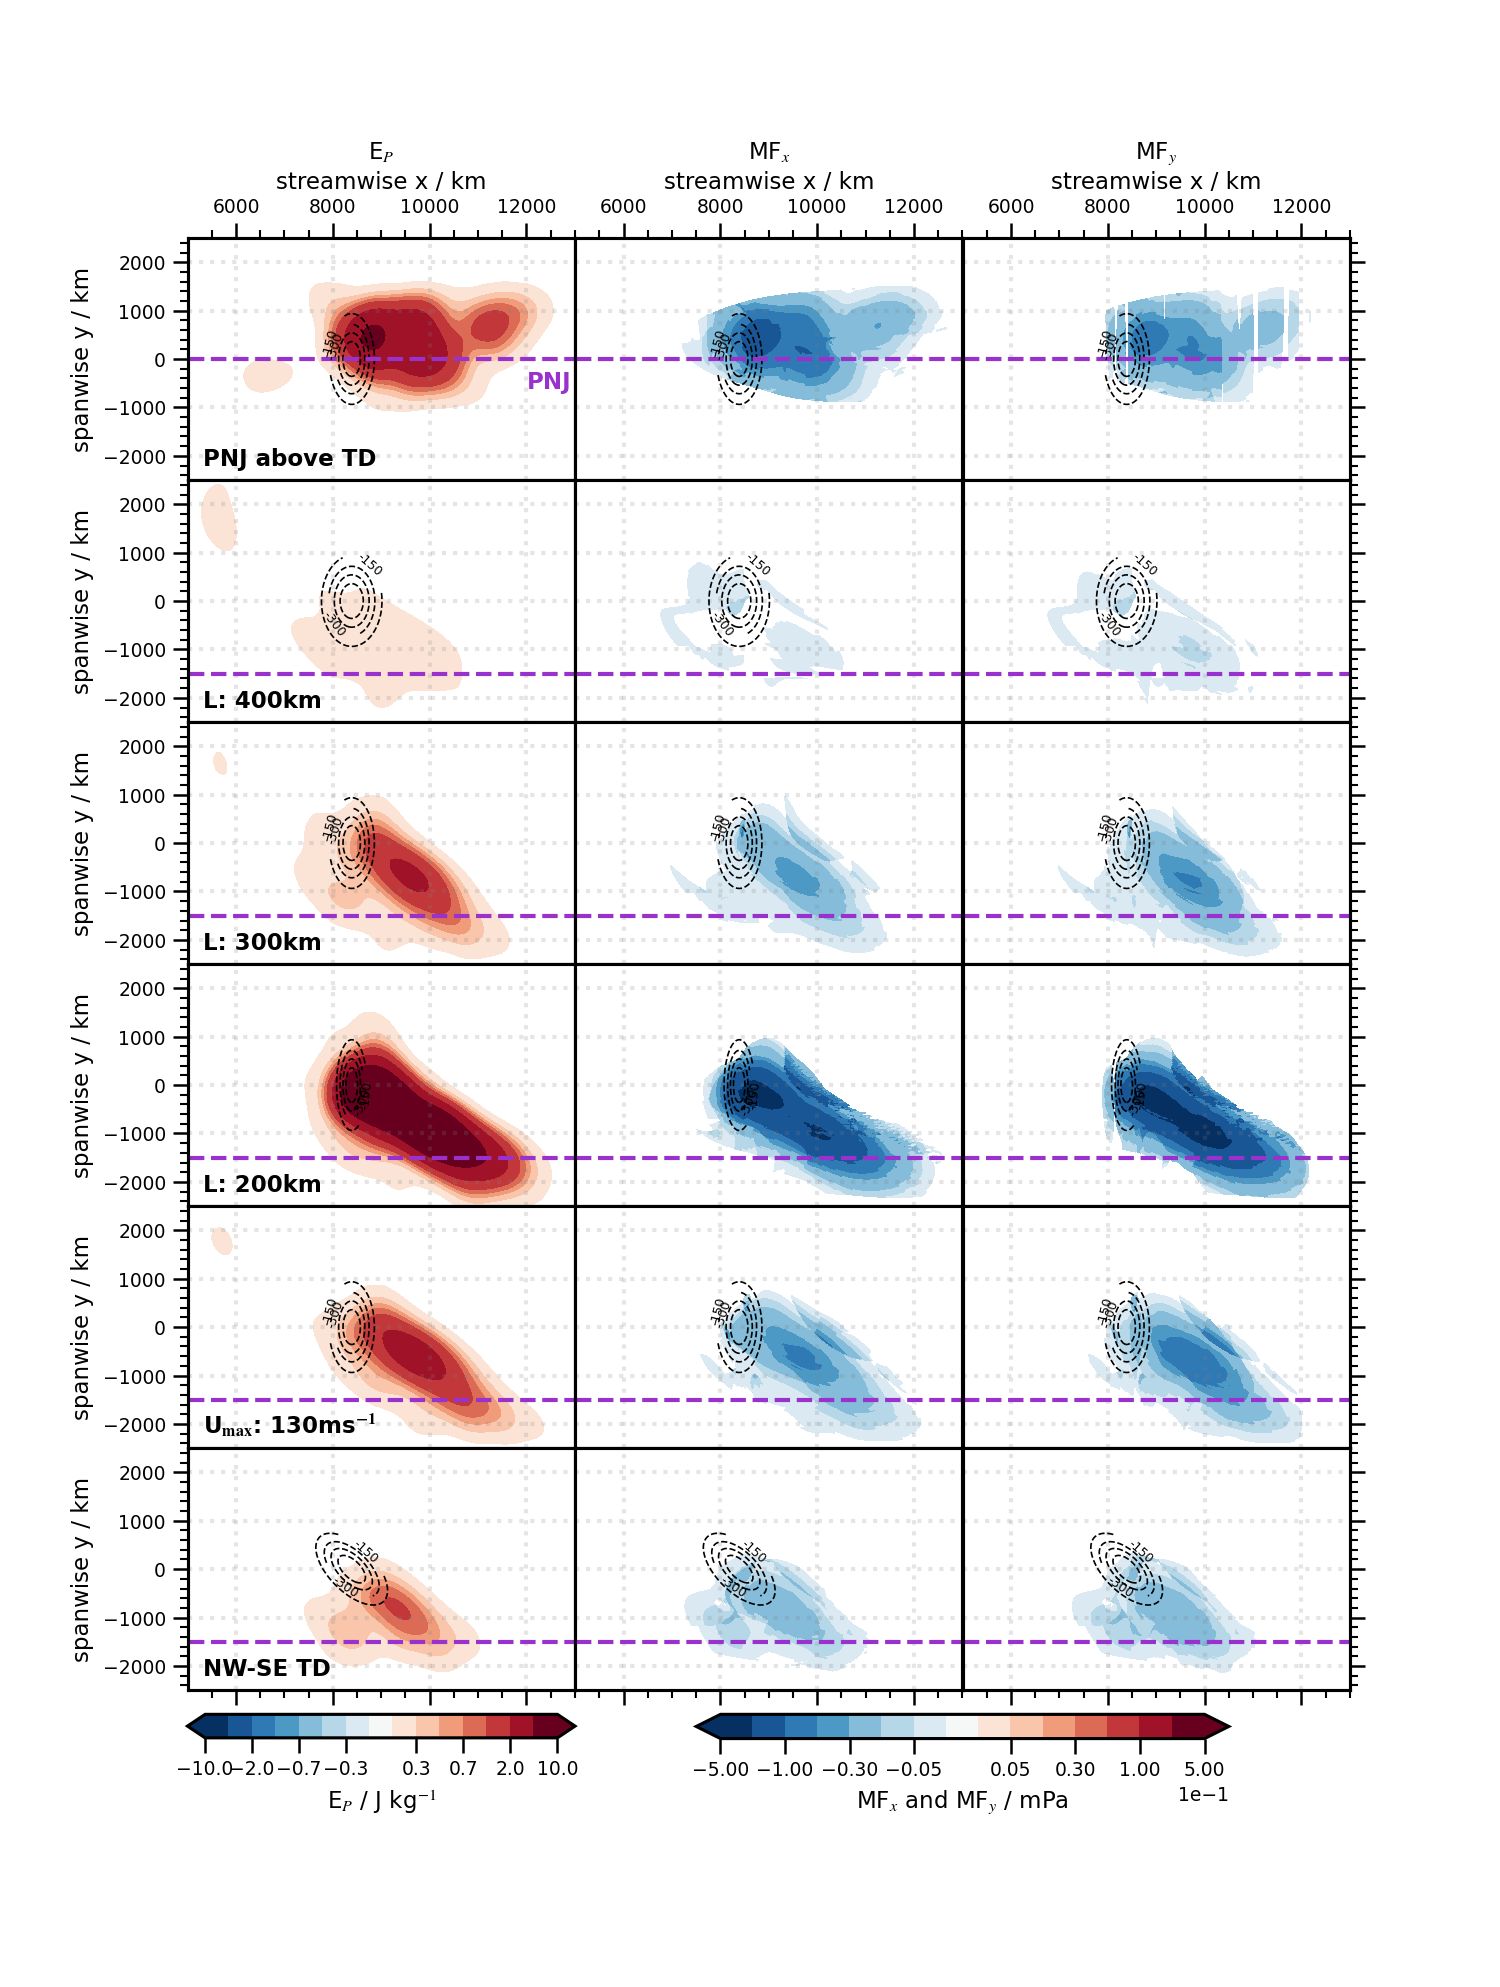
\includegraphics[width=0.99\textwidth]{figures_3D/waveletAna_fluxes_obs.png}
    \caption{Horizontal cross sections at 40km above the tropopause for five simulations with horizontal and meridional shear in a barotropic environment. Shown are $\theta$', $\lambda_x$ and $\lambda_y$ at 72h into the simulation. Dominant zonal and meridional wavelengths for each grid point are determined from wavelet analysis.}
    \label{fig:waveletAna_dudy}
\end{figure*}


\section{Transient lower surface boundary in quiescent fluid}
% simulations without Coriolis in 2D

move and stop 

show how wave propagate -> observe energy propagation / phase lines... 



\section{EULAG setup for idealized Q3D and 3D simulations}

EULAG provides multiple options to define background states of the atmosphere. For the presented simulations vertical ambient profiles define an isothermal atmosphere with constant stability as described by \textcite{bacmeister_breakdown_1989}. These exponential profiles of potential temperature and density avoid physical restrictions towards higher altitudes and are thus well suited for the investigation of deep gravity wave propagation. Defining a potential temperature and density scale height $H_{\Theta}$ and $H_{\rho}$ leads to

\begin{equation}
\begin{aligned}
    p_0(z) &= p_{00} e^{-\frac{z}{H_{\rho}}} \quad \textrm{with} \quad H_{\rho} = \frac{R_d}{c_p} H_{\Theta} = \frac{R_d T_{00}}{g} \\
    \rho_0(z) &= \frac{p_0(z)}{R_d T_{00}} = \rho_{00} e^{-\frac{z}{H_{\rho}}} \\
    T_0(z) &= \frac{p_{00}}{R_d \rho_{00}} \\
    \Theta_0(z) &= T_{00} \frac{p_{00}}{p}^{\kappa} \\
    \Theta_0(z) &= T_{00} e^{\frac{z}{H_{\Theta}}} \quad \textrm{with} \quad H_{\Theta} = \frac{g}{N^2} \\
    \label{equ:ambient-Profiles}
\end{aligned}
\end{equation}
% based on hydrostatic approximation dp/dz = -rho*g -> pressure with density scale height

with the Brunt-Vaisala frequency $N$, the specific gas constant $R_d$ and the specific heat capacity at constant pressure $c_p$. $p_0$, $\rho_0$ and $T_0$ represent a reference state of the atmosphere.

\begin{table*}[ht]
\centering
\caption{Ambient profile parameters and reference state of the atmosphere for simulations of the troposphere for model validation and of the stratosphere}


Include Figure of environmental profiles for simulations of stratosphere!!!


\begin{tabular}{@{}cccc@{}}
\toprule
 & Unit & Troposphere & Stratosphere \\ \midrule[1pt]

$g$ & m s$^{-2}$ & 9.80616 & 9.80616 \\
$R$ & J kg$^{-1}$ K$^{-1}$ & 287.04 & 287.04 \\
$c_p$ & J kg$^{-1}$ K$^{-1}$ & $3.5 R$ & $3.5 R$ \\
$p_{00}$ & Pa & $1.01 \cdot 10^5$ & $0.235 \cdot 10^5$ \\
$\rho_{00}$ & kg m$^{-3}$ & 0.3676 (1.2856) & 0.3454 \\
$T_{00}$ & K & 957.17 (273.69) & 239.39 \\
$N$ & s$^{-1}$ & 0.01 & 0.02 \\
$H_{\rho}$ & m & 28017.6 (8011.3)  & 7004.4 \\
$H_{\Theta}$ & m & 98061.6 & 24515.4  \\

\bottomrule
\end{tabular}
\label{tab:ambientProfiles}
\end{table*}

Should density scale height fit to reference state or should it rather relate correctly to stability / theta scale height based on two atomic gases? This results in temperature around 900K...
Value of density scale height effects

For stratosphere simulations it s fully consistent!!! 

- full 3D simulations (cite zhang.. 2005 together with Alexander/Durran...) extend those simulations to upper stratosphere.



